% Chapter 1

\chapter{Introduction} % Main chapter title

\label{Chapter1} % For referencing the chapter elsewhere, use \ref{Chapter1} 

%----------------------------------------------------------------------------------------

% Define some commands to keep the formatting separated from the content 
\newcommand{\keyword}[1]{\textbf{#1}}
\newcommand{\tabhead}[1]{\textbf{#1}}
\newcommand{\code}[1]{\texttt{#1}}
\newcommand{\file}[1]{\texttt{\bfseries#1}}
\newcommand{\option}[1]{\texttt{\itshape#1}}

\newcommand{\mfg}{manufacturer}

\section{Goals}

%----------------------------------------------------------------------------------------

\section{Methods}

%----------------------------------------------------------------------------------------

\section{Safety-critical devices}
\subsection{What are safety-critical devices?}
% TODO Maybe already mention real-time requirements
The failure or malfunction of a safety-critical system has the potential to cause one or more of the following outcomes [source]:
\begin{itemize}
\item injury or death
\item damage to property
\item environmental harm
\end{itemize}
A safety-critical device is consequently an embedded device with a dedicated function that has the above mentioned property. Such a device has to at least contain dedicated hardware but may also have mechanical and/or software components.

% TODO ISO 14971 source
The legal entity responsible for designing and manufacturing the device will be referred to as \mfg{}, in accordance with ISO 1497. 
\subsection{Basic concepts}
\subsubsection{Safety regulations}
% REWRITE Sounds a bit bad
The main goal of safety-critical device manufacturers is to create a safe device. This protects them from expensive lawsuits and can give them a competitive advantage.

% TODO Think about more commonalities and maybe refactor this
However, in most markets, a favourable real-world safety alone is not enough to gain permission to sell the device.  Each market (medical, nuclear, aviation etc.) and regulatory body (EU, US etc.) has their own standard for normative safety that needs to be met. This thesis will lean mostly on IEC 61508  because it represents a general standard from which many others derive. And although there are important differences that need to be kept in mind, for the purpose of this thesis the standards are similar enough to be interchangeable. [source?]

The specific instructions and level of rigour differ between the standards but they usually share the following requirements:

\begin{itemize}
\item A compliant quality management system needs to be used
\item Device requirements need to be analyzed
\item Requirements need to be verified
\item Unreasonable risk needs to be reduced
\item Extensive documentation on all aspects of design and manufacturing
\end{itemize}

In most standards it is not enough to show that the end product is safe, the \mfg{} also has to present the documents that he generated along the way to the authorities. There are exceptions to this rule if third-party or legacy parts are used but these need to be justified as well. Therefore it is usually infeasible to certify a device after the development process, if it was not designed with certification in mind. [source]

A failed certification attempt is undesirable, as it is associated with additional cost and time but it is also not a death sentence for the device. The regulatory body will point out the problems and give the \mfg{} the option to fix them and resubmit the device for certification.

The rigour that is demanded by regulatory bodies is dependent on the risk category that can be assigned to a device. These risk categories will be called \keyword{criticality levels} from here on out. 

\subsubsection{Criticality levels}
% TODO explain what they are and source

% NOTE Do I gloss over this point too much? Or should it be mentioned here in the first place?
No matter what definition of criticality levels is chosen, they all share some properties that guide the rest of this thesis: A function with a higher criticality level is more expensive to implement and verify than one with a lower level. because there is more documentation effort, more rigorous risk analysis and so on. Two units of a device are only allowed to have differing criticality levels, if there is sufficient evidence that the higher criticality function is independent from the lower criticality function [source]. 

This constellation of heterogeneous criticality levels within the device is very common and usually referred to as mixed criticality. Its motivations and problems will be explored in the next section.
\subsection{Mixed criticality}
\subsubsection{Motivations}
The core motivation for assigning different criticality levels within a device has already been mentioned; it is cheaper to implement and verify a low criticality part. But this is not the only motivation, as it only applies to functionality that is implemented by the \mfg{} and not by a third-party .

% NOTE Get a hardware perspective
* This is all under the assumption that a case for lower criticality can be made in the first place. If the USB stack for example is required for a function that has a high non-reducible criticality, the USB stack needs to be certified.
* Focusing on software in this section
* Third-party software that has been developed with safety in mind does exist (certified USB stack for example)
* However these are more expensive and because they have a narrow target audience, there is not much variety or special functionality
* Whereas Linux has much free and open source software with a large user base and extensive functionality. It is however usually infeasible to verify Linux and the associated software
* In these cases the benefit is more drastic than saving some money on verification, some functionality can become feasible in the first place through mixed criticality
* At the same time [Roy source] user demands are getting more sophisticated along with device power. But reinventing the wheel (or advanced GUI with touch controls) is expensive and time consuming.

% TODO Cite the study that Roy used in his business case
\subsubsection{Problems}
% NOTE Make sure the point I reiterate here is clearly made in the previous section
Now it is clear why mixed criticality is actually a desirable property in a lot of devices. It can save cost and time, as well as provide functionality that would have been infeasible to realize without. 

However, as alluded to earlier, mixed criticality does not come without problems. Regulatory standards require [source IEC-61508 part 1 and 2] sufficient evidence for independence between functions of different criticality be shown to them. If \mfg{} can not provide this evidence all functions need to comply to the highest criticality level.

Sufficient independence is given, if it can be shown that a dependent failure between the higher and lower criticality function is sufficiently low in the context of the highest level.
To achieve this a system architecture is required that can reliably separate components. The precise requirements this separation architecture needs to fulfill will be tackled in the next section.

%----------------------------------------------------------------------------------------

\section{The separation architecture}
% TODO Cite Wittenstein white papers
% NOTE Think about where and how to mention real-time requirements
There are four attributes the separation architecture needs to solve the mixed criticality problem.
\subsection{Spatial separation}

\begin{comment}
\begin{figure}
\centering
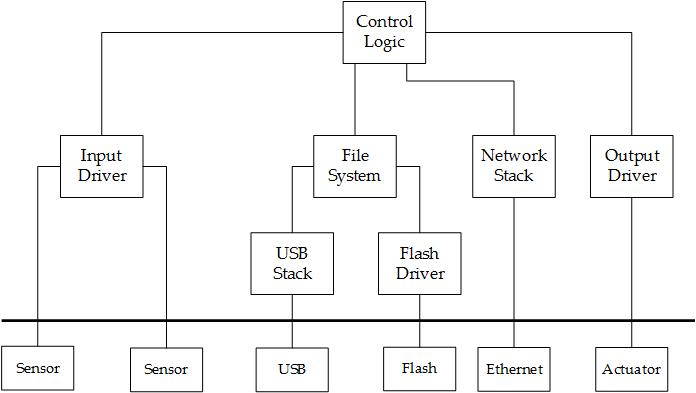
\includegraphics{Figures/Drawing1}
\decoRule
\caption{Test}
\label{fig:sepArch}
\end{figure}
\end{comment}

Spatial separation means that access of physical resources cannot lead to conflicts or corruption. This includes memory access as well as system resources such as hardware peripherals. 

If shared access to any system resources is necessary, some kind of arbiter needs to be in place to give consistent access to components. 
\subsection{Temporal separation}
Temporal separation is achieved, if it is impossible for any system software to compromise the processing demands of another.
Managing access to available processing resources is the main part of temporal separation. However, system events and triggers may also require analysis. Excessive interrupt routine run time, for example, can cause processing resources to be unavailable to the main system. 
\subsection{Data integrity and validity}
Data passed through unsafe components has to be either not safety related or protected. Whereas protection refers to ensuring the data's integrity and validity after it has passed through the unsafe components and before it is used in safety related processing.

In practice this doesn't have to be part of the architecture but may be handled in the application software. Nevertheless it is an important aspect that needs to be kept in mind.
\subsection{Certifiable compliance}
It may not come as a surprise that the separation architecture also needs to fulfill these requirements in the eyes of the regulatory bodies, as they are the reason for the architecture's inception.
How this may be achieved differs based on architecture and standard but it needs to be feasible at the very least.

%----------------------------------------------------------------------------------------

\section{Existing architectures}
\subsection{Embedded operating systems}
Apart from bare-metal software, which is reserved for the most trivial cases,  embedded operating systems are the simplest approach to device architecture. 
\subsubsection{GPOS}
* Spatial separation is possible (with MMU)
* Temporal separation is typically not possible. In fact the core design principles counteract real-time determinism
* Whether or not real-time requirements can be hit is debatable even with modifications that theoretically enable this.
* They are usually huge code bases that can't be feasibly certified (Roche Linux appears to be a counter example)
* Independence and interference freeness are problematic
\subsubsection{RTOS}
* There are probably options that can provide adequate temporal and spatial separation. Where spatial is often a bigger concern
* These solutions are often very expensive 
* Application complexity can be limited
	* by lack of varied and high-quality software like GUI frameworks
    * by the restrictions imposed by the architecture
 * Current scheduling solutions also promote "scheduling slack"
 * Currently multicore support is limited
\subsection{AMP}
Multi
\subsection{Hardware supervised AMP}
\subsection{Hardware separated subsystems}

%----------------------------------------------------------------------------------------

\section{Embedded safety hypervisor origins}
\subsection{Virtualization}
\paragraph{Paravirtualization}
\paragraph{Full virtualization}
\subsection{Original hypervisor use case}
\subsection{Microkernels}
\subsection{Unification of the two concepts}


